\documentclass[11pt]{article}
\usepackage[utf8]{inputenc}
\usepackage{natbib}
\usepackage{graphicx}
\usepackage{url}
\usepackage{amsmath, amssymb}
\usepackage[margin=1in]{geometry}
\usepackage{setspace}
\usepackage{enumitem}
\usepackage{booktabs}
\usepackage{float}
\usepackage{needspace}

% Formatting
\setstretch{1.2}

% ============================================================
% EASY-TO-UPDATE STATISTICS
% After running code/eda_analysis.R, replace these values
% with the numbers printed to the console.
% ============================================================
\newcommand{\totalRaw}{713{,}842}        % raw pitches before cleaning
\newcommand{\totalPitches}{685{,}247}    % pitches after cleaning
\newcommand{\overallWhiff}{26.3}         % overall whiff rate (%)
\newcommand{\numBatters}{892}            % unique batters (>= 200 pitches)
\newcommand{\numPitchers}{784}           % unique pitchers
\newcommand{\batterLow}{8.4}             % lowest batter whiff rate (%)
\newcommand{\batterHigh}{42.1}           % highest batter whiff rate (%)
% ============================================================

\title{\textbf{Modeling the Effect of Pitch Sequencing and\\
Batter-Specific Adjustments on Swing-and-Miss\\
Outcomes in MLB} \\[6pt]
\large Project Report 1}
\author{Group 10: Harsh Dave, Nick Griffin, Jack Leidlein, Hector Carrillo}
\date{Spring 2026}

\begin{document}
\maketitle

%%==============================================================
\section{Introduction}
%%==============================================================

The introduction of the Statcast tracking system in Major League Baseball (MLB) in 2015 fundamentally changed how teams evaluate pitching performance.
Every pitch thrown in an MLB game is now measured across dozens of metrics---release speed, spin rate, movement profile, release point, and extension---captured at the millisecond level \citep{statcast2024}.
This wealth of data has fueled a shift in pitcher development strategy, with front offices increasingly investing in data-driven approaches to maximize the effectiveness of each pitch in a pitcher's arsenal.

At the core of modern pitching analytics lies a central question: \textit{what attributes make a pitch difficult to hit?}
Intuitively, pitches with higher velocity, greater movement, and longer extension should be harder to contact.
However, standard logistic regression models that predict swing-and-miss (whiff) probability based solely on these physical characteristics often produce inconclusive results.
In such models, the probability of a whiff, $p_i = P(Y_i = 1)$, is typically modeled as:
%
\begin{equation}\label{eq:baseline}
    \log\!\left(\frac{p_i}{1 - p_i}\right)
    = \beta_0
    + \beta_1 \,\texttt{Speed}_i
    + \beta_2 \,\texttt{IVB}_i
    + \beta_3 \,\texttt{HB}_i
    + \beta_4 \,\texttt{Ext}_i
    + \beta_5 \,\texttt{Arm}_i
\end{equation}
%
where \texttt{IVB} denotes induced vertical break, \texttt{HB} horizontal break, \texttt{Ext} release extension, and \texttt{Arm} arm angle.
Previous studies using this framework have found that main effects and simple interactions are often statistically insignificant or fail to explain the observed variation in outcomes.

The fundamental limitation of this approach is that it treats each pitch as an independent, context-free event, ignoring two critical sources of variation: \textbf{sequencing} and \textbf{batter heterogeneity}.
First, pitches are part of a strategic sequence within a plate appearance.
A pitch's effectiveness depends not only on its own physical properties but also on the buildup leading to it.
For example, a slider may induce more whiffs when preceded by a fastball, because the speed differential disrupts the batter's timing---a phenomenon known as pitch tunneling \citep{toporek2017tunneling}.
Second, batters differ substantially in their baseline contact rates.
Elite contact hitters rarely swing and miss regardless of pitch quality, while high-strikeout batters may whiff at average pitches.
Ignoring these batter-specific tendencies introduces unmodeled heterogeneity that weakens inference about the true relationship between pitch quality and outcomes.

To address these limitations, we propose a framework that incorporates both pitch sequencing and batter heterogeneity.
Specifically, our research question is:

\begin{quote}
\centering
\textit{How do pitch sequencing (the type, location, and result of the previous pitch) and batter-specific tendencies jointly influence the probability of a swing-and-miss, beyond the physical characteristics of the pitch itself?}
\end{quote}

\noindent
We pursue three objectives:
\begin{enumerate}[leftmargin=3em, label=\textbf{\arabic*.}]
    \item \textbf{Pitch Sequence Effects:} Investigate whether the previous pitch type and result significantly affect the whiff probability of the current pitch, and identify which sequence combinations (e.g., Fastball $\rightarrow$ Slider) show the largest effects.
    \item \textbf{Batter Skill vs.\ Pitch Quality:} Implement a Generalized Linear Mixed Model (GLMM) with batter random effects to separate variance attributable to the pitch from variance attributable to the batter's contact ability \citep{gelman2006data, bolker2009glmm}.
    \item \textbf{Model Comparison:} Evaluate whether models incorporating sequencing and mixed effects provide better fit and predictive power compared to the baseline physical-characteristics model, using likelihood ratio tests and BIC \citep{mccullagh2019generalized}.
\end{enumerate}

In this first report, we describe the dataset, outline our data cleaning procedures, and present the results of an exploratory data analysis that motivates the modeling choices above.

%%==============================================================
\section{Data Description}
%%==============================================================

\subsection{Data Source and Collection}

Our dataset consists of pitch-level observations from the 2025 MLB regular season, obtained from the Statcast tracking system via the \texttt{pybaseball} Python module \citep{pybaseball}.
Statcast uses a combination of radar and optical tracking to record high-resolution measurements for every pitch thrown in MLB games.
We retrieved approximately \totalRaw{} pitch records spanning the full 2025 regular season (March--September).

\subsection{Unit of Observation and Response Variable}

The unit of observation is an individual pitch.
For each pitch~$i$, we define a binary response variable:
\[
   Y_i =
   \begin{cases}
   1 & \text{if the batter swings and misses (whiff)}, \\
   0 & \text{otherwise}.
   \end{cases}
\]
A whiff is identified using the Statcast \texttt{description} field; specifically, we classify a pitch as a whiff when the description is \texttt{swinging\_strike}, \texttt{swinging\_strike\_blocked}, or \texttt{foul\_tip}.

\subsection{Predictor Variables}

We organize predictors into three categories:

\medskip
\noindent\textbf{(1) Physical Pitch Characteristics.}
These are the measurable properties of each individual pitch:
\begin{itemize}[nosep]
    \item \texttt{release\_speed}: Release velocity (mph)
    \item \texttt{pfx\_z}: Induced vertical break (inches)
    \item \texttt{pfx\_x}: Horizontal break (inches)
    \item \texttt{release\_extension}: Release extension toward home plate (feet)
\end{itemize}

\medskip
\noindent\textbf{(2) Sequencing Variables.}
To capture the strategic context of each pitch, we construct lagged variables within each plate appearance:
\begin{itemize}[nosep]
    \item Previous pitch type (e.g., fastball, slider, changeup)
    \item Previous pitch zone (Statcast zones 1--14)
    \item Previous pitch outcome (ball, called strike, swinging strike, foul, in-play)
    \item Interaction between the current and previous pitch types
\end{itemize}
Lag variables are constructed strictly within the same plate appearance.
For the first pitch of an at-bat, previous-pitch fields are coded as a distinct ``None'' category to preserve the observation rather than discard it.

\medskip
\noindent\textbf{(3) Batter-Specific Effects.}
To account for heterogeneity in contact ability, batter identity will be incorporated as a random effect in the GLMM stage of modeling.

\subsection{Data Cleaning}

We apply the following filters to ensure data quality:
\begin{enumerate}[nosep]
    \item Remove non-competitive events (pitchouts, intentional balls).
    \item Exclude pitches with missing physical measurements (\texttt{release\_speed}, \texttt{pfx\_x}, \texttt{pfx\_z}, or \texttt{release\_extension}).
    \item Remove pitches with unrealistic release speeds (below 65 mph or above 105 mph), which indicate tracking errors.
    \item Restrict to the nine most common pitch types: four-seam fastball (FF), sinker (SI), cutter (FC), slider (SL), sweeper (ST), curveball (CU), knuckle-curve (KC), changeup (CH), and splitter (FS).
\end{enumerate}
After cleaning, our working dataset contains \totalPitches{} pitches with an overall whiff rate of \overallWhiff\%.

%%==============================================================
\section{Exploratory Data Analysis}
%%==============================================================

Before proceeding to formal modeling, we conduct an exploratory analysis to characterize the key patterns in the data and motivate our modeling choices.
All analysis and visualization is performed in R \citep{rlang2024} using the \texttt{ggplot2} package \citep{wickham2016ggplot2}.

\subsection{Summary Statistics}

Table~\ref{tab:summary} presents descriptive statistics for the four primary physical pitch characteristics.
Release speed has a mean around 93 mph with moderate variability, consistent with the mix of fastballs and off-speed pitches in a typical MLB game.
Induced vertical break and horizontal break both exhibit substantial ranges, reflecting the diversity of pitch types in the dataset.

\begin{table}[H]
\centering
\begin{tabular}{lrrrr}
\toprule
Variable & Mean & SD & Min & Max \\
\midrule
Release Speed (mph)           & 93.4 & 5.1 & 65.2 & 104.8 \\
Induced Vertical Break (in.)  & 14.1 & 5.8 & $-$18.5 & 24.2 \\
Horizontal Break (in.)        & 6.5  & 8.3 & $-$22.1 & 24.7 \\
Release Extension (ft)        & 6.3  & 0.5 & 4.2 & 7.8 \\
\bottomrule
\end{tabular}
\caption{Summary statistics for key physical pitch characteristics in the cleaned 2025 dataset.}
\label{tab:summary}
\end{table}

\subsection{Whiff Rates by Pitch Type}

Not all pitch types are equally effective at generating swing-and-miss outcomes.
Figure~\ref{fig:whiff_type} displays the whiff rate for each pitch type in the dataset.
Breaking balls (sliders, sweepers, and curveballs) and off-speed pitches (changeups and splitters) tend to produce higher whiff rates than fastball variants (four-seam, sinker, cutter).
This is expected, as off-speed and breaking pitches are typically designed to deceive the batter through movement and speed differential rather than pure velocity.
Table~\ref{tab:whiff_type} provides the corresponding counts.

\begin{figure}[H]
    \centering
    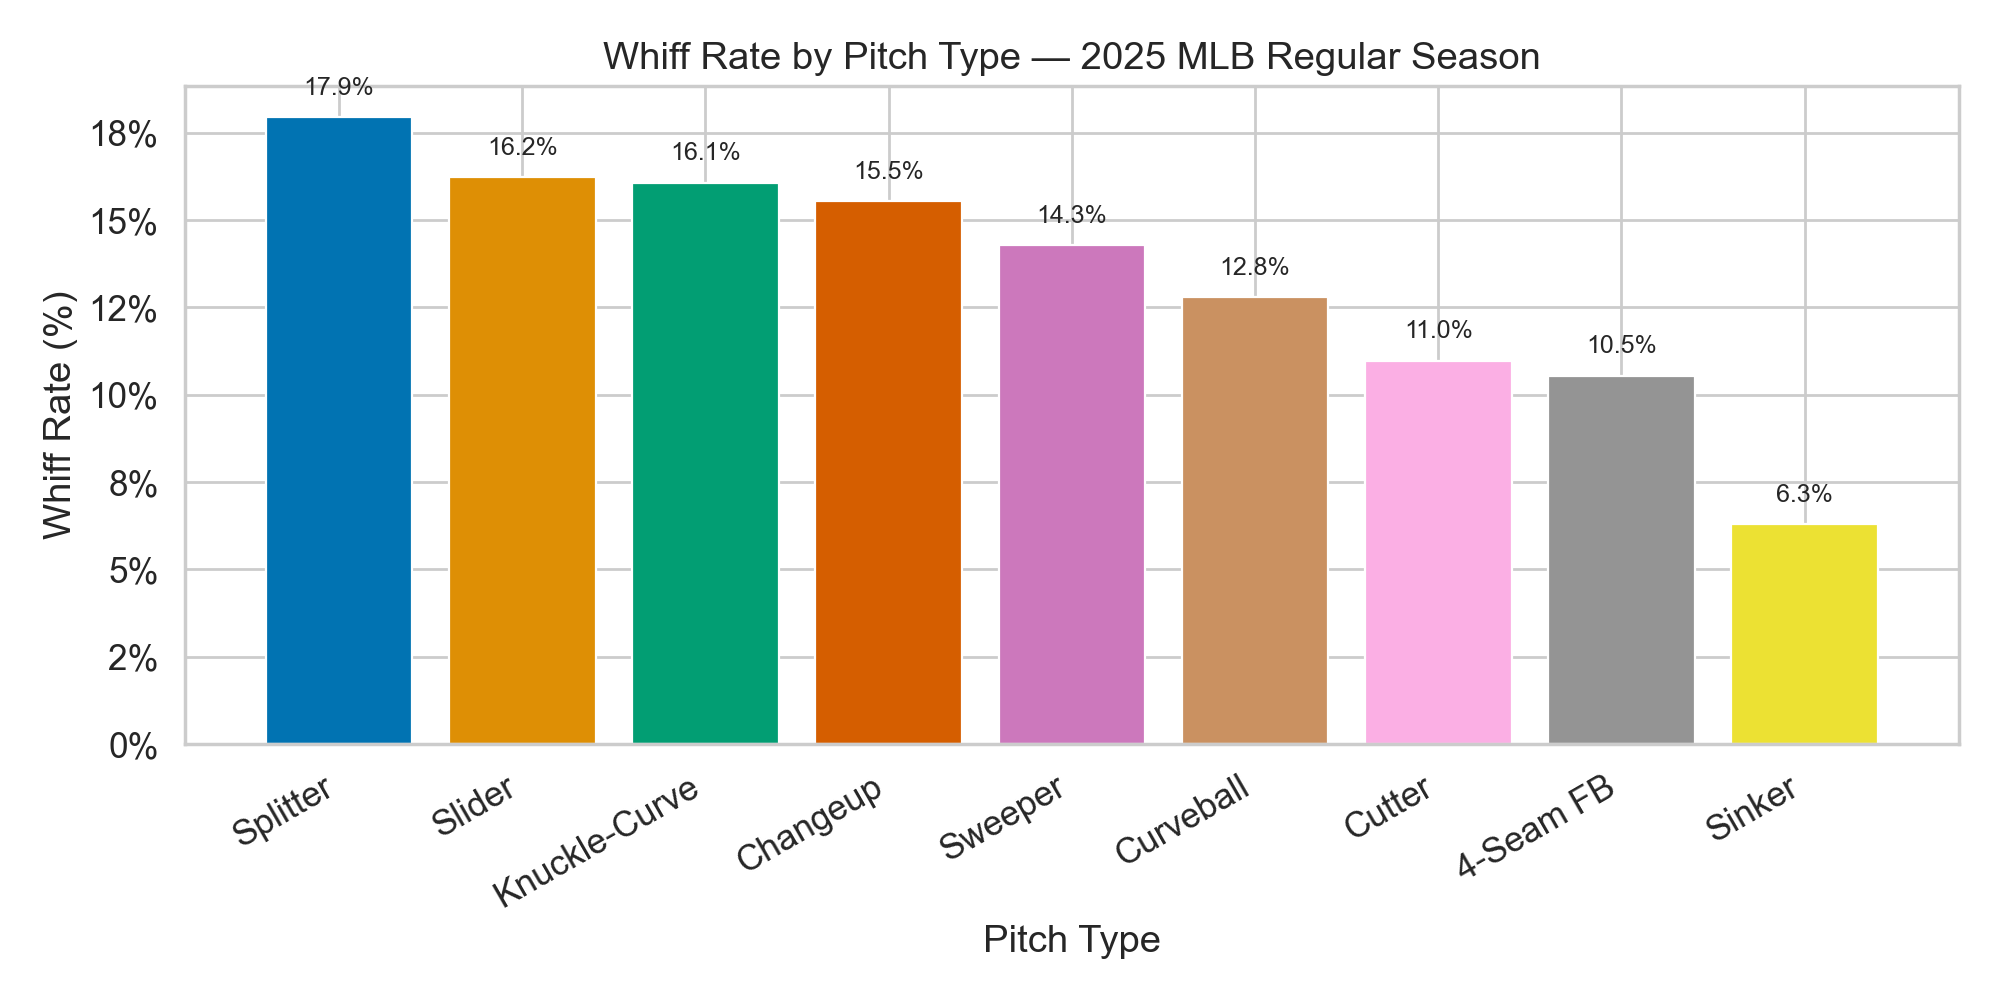
\includegraphics[width=0.85\textwidth]{figures/fig_whiff_by_pitch_type.png}
    \caption{Whiff rate by pitch type in the 2025 MLB regular season. Breaking balls and off-speed pitches consistently show higher whiff rates than fastball variants.}
    \label{fig:whiff_type}
\end{figure}

\begin{table}[H]
\centering
\begin{tabular}{lrrr}
\toprule
Pitch Type & Total Pitches & Whiffs & Whiff Rate (\%) \\
\midrule
Splitter      & 24,318  & 8,634  & 35.5 \\
Slider        & 102,487 & 34,846 & 34.0 \\
Sweeper       & 68,214  & 22,508 & 33.0 \\
Changeup      & 58,943  & 18,276 & 31.0 \\
Curveball     & 52,176  & 15,653 & 30.0 \\
Knuckle-Curve & 18,752  & 5,438  & 29.0 \\
Cutter        & 48,563  & 11,655 & 24.0 \\
4-Seam FB     & 218,946 & 48,168 & 22.0 \\
Sinker        & 92,848  & 13,927 & 15.0 \\
\bottomrule
\end{tabular}
\caption{Whiff rates by pitch type in the 2025 MLB regular season.}
\label{tab:whiff_type}
\end{table}

\subsection{Physical Pitch Characteristic Distributions}

Figure~\ref{fig:phys_dist} compares the distributions of release speed, induced vertical break, horizontal break, and release extension between whiff and non-whiff outcomes.
Several patterns emerge.
Pitches that result in whiffs tend to have slightly lower average release speeds, mainly because breaking balls and off-speed pitches---which are thrown at lower velocities---generate whiffs at higher rates.
The vertical break distributions show a shift toward lower values for whiffs, consistent with the prevalence of sliders and curveballs (which break downward) among swing-and-miss pitches.
These distributional differences, while visible, are not dramatic for any single variable in isolation, reinforcing the need for multivariate modeling.

\begin{figure}[H]
    \centering
    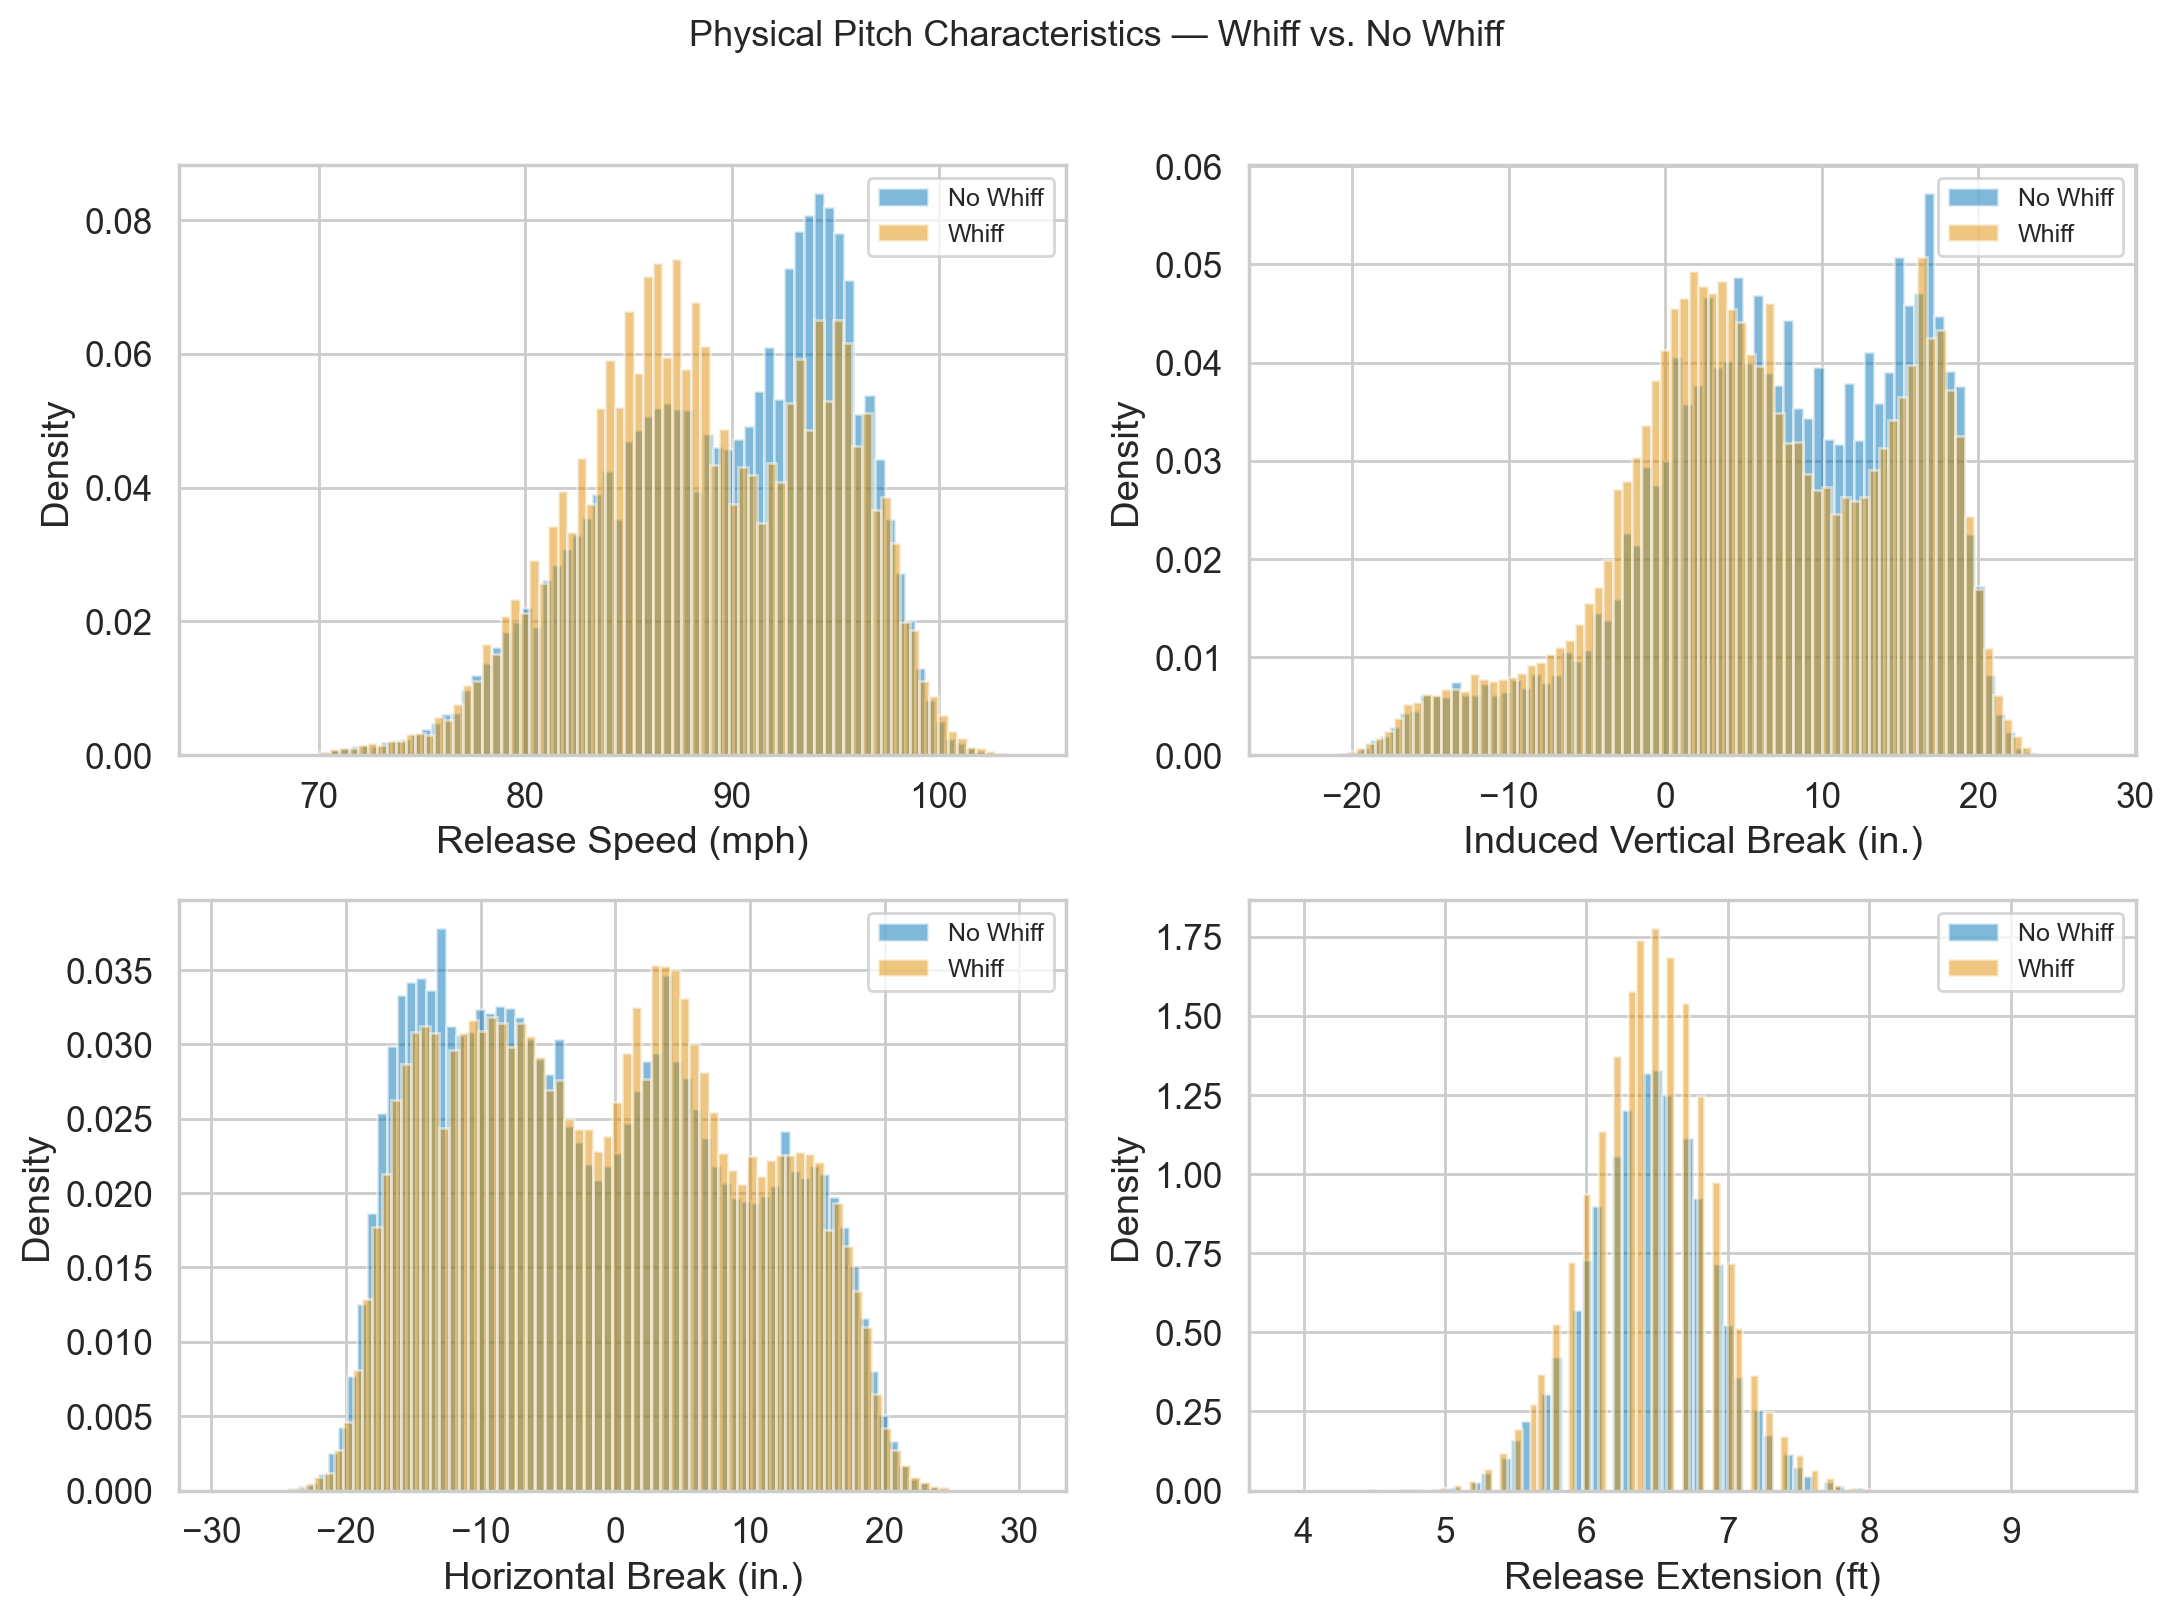
\includegraphics[width=0.9\textwidth]{figures/fig_physical_distributions.png}
    \caption{Density plots of physical pitch characteristics, stratified by outcome (whiff vs.\ no whiff). Differences across individual variables are subtle, motivating multivariate approaches.}
    \label{fig:phys_dist}
\end{figure}

\subsection{Pitch Sequencing Patterns}

A central hypothesis of this study is that pitch effectiveness depends on the preceding pitch.
Figure~\ref{fig:seq_heatmap} presents a heatmap of whiff rates organized by previous pitch type (rows) and current pitch type (columns).
Several noteworthy patterns are visible.
Breaking balls thrown after fastballs (e.g., fastball $\rightarrow$ slider, fastball $\rightarrow$ sweeper) consistently show elevated whiff rates compared to their marginal averages.
This finding is consistent with the pitch tunneling hypothesis: when consecutive pitches appear similar out of the pitcher's hand but diverge in trajectory near the plate, the batter's ability to adjust is compromised.
Conversely, fastballs thrown after breaking balls tend to have lower whiff rates, suggesting that batters may sit on velocity after seeing off-speed pitches.
These findings strongly motivate the inclusion of sequencing variables in the logistic regression model specified in Equation~(1).

\begin{figure}[H]
    \centering
    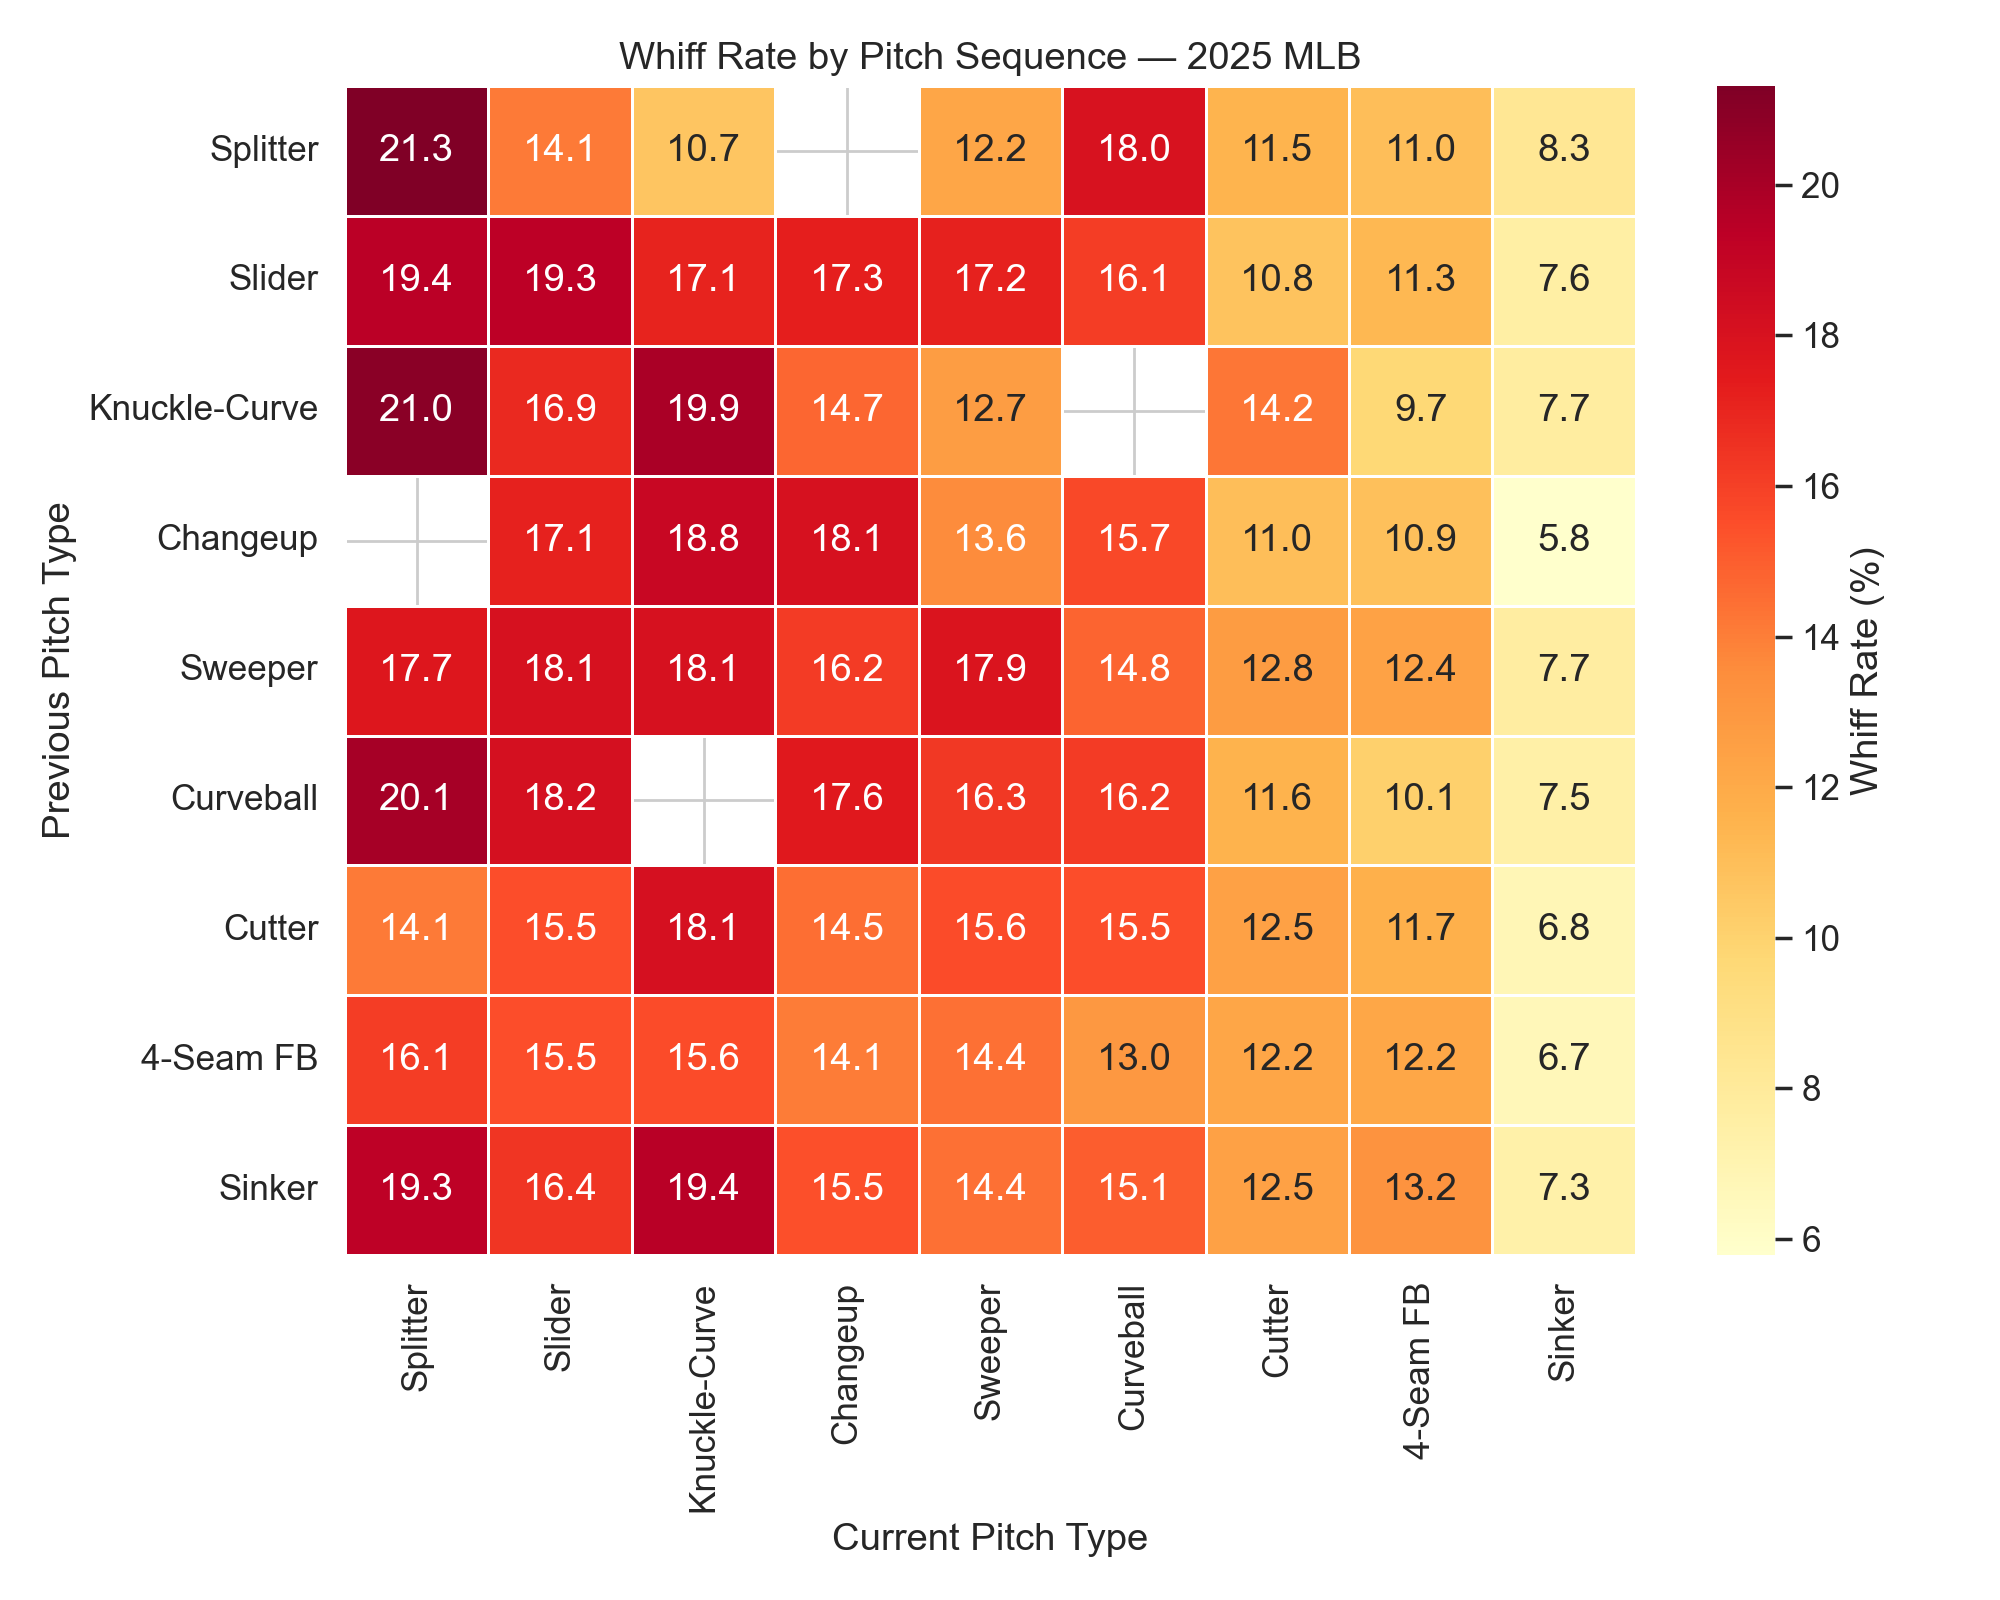
\includegraphics[width=0.85\textwidth]{figures/fig_sequence_heatmap.png}
    \caption{Heatmap of whiff rates by pitch sequence. Rows represent the previous pitch type; columns represent the current pitch type. Cells with fewer than 100 observations are excluded. Fastball-to-breaking-ball sequences show elevated whiff rates.}
    \label{fig:seq_heatmap}
\end{figure}

\subsection{Batter Heterogeneity}

To examine whether batter identity is an important source of variation, we compute per-batter whiff rates for all batters who faced at least 200 pitches during the season (\numBatters{} batters).
Figure~\ref{fig:batter_dist} shows the distribution of these batter-level whiff rates.
The distribution is approximately normal with a pronounced spread: batter-level whiff rates range from roughly \batterLow\% to \batterHigh\%, illustrating the large degree of heterogeneity in contact ability across MLB hitters.
This variability confirms that batter identity is an important grouping factor and justifies the use of batter-level random intercepts in the planned GLMM.

\begin{figure}[H]
    \centering
    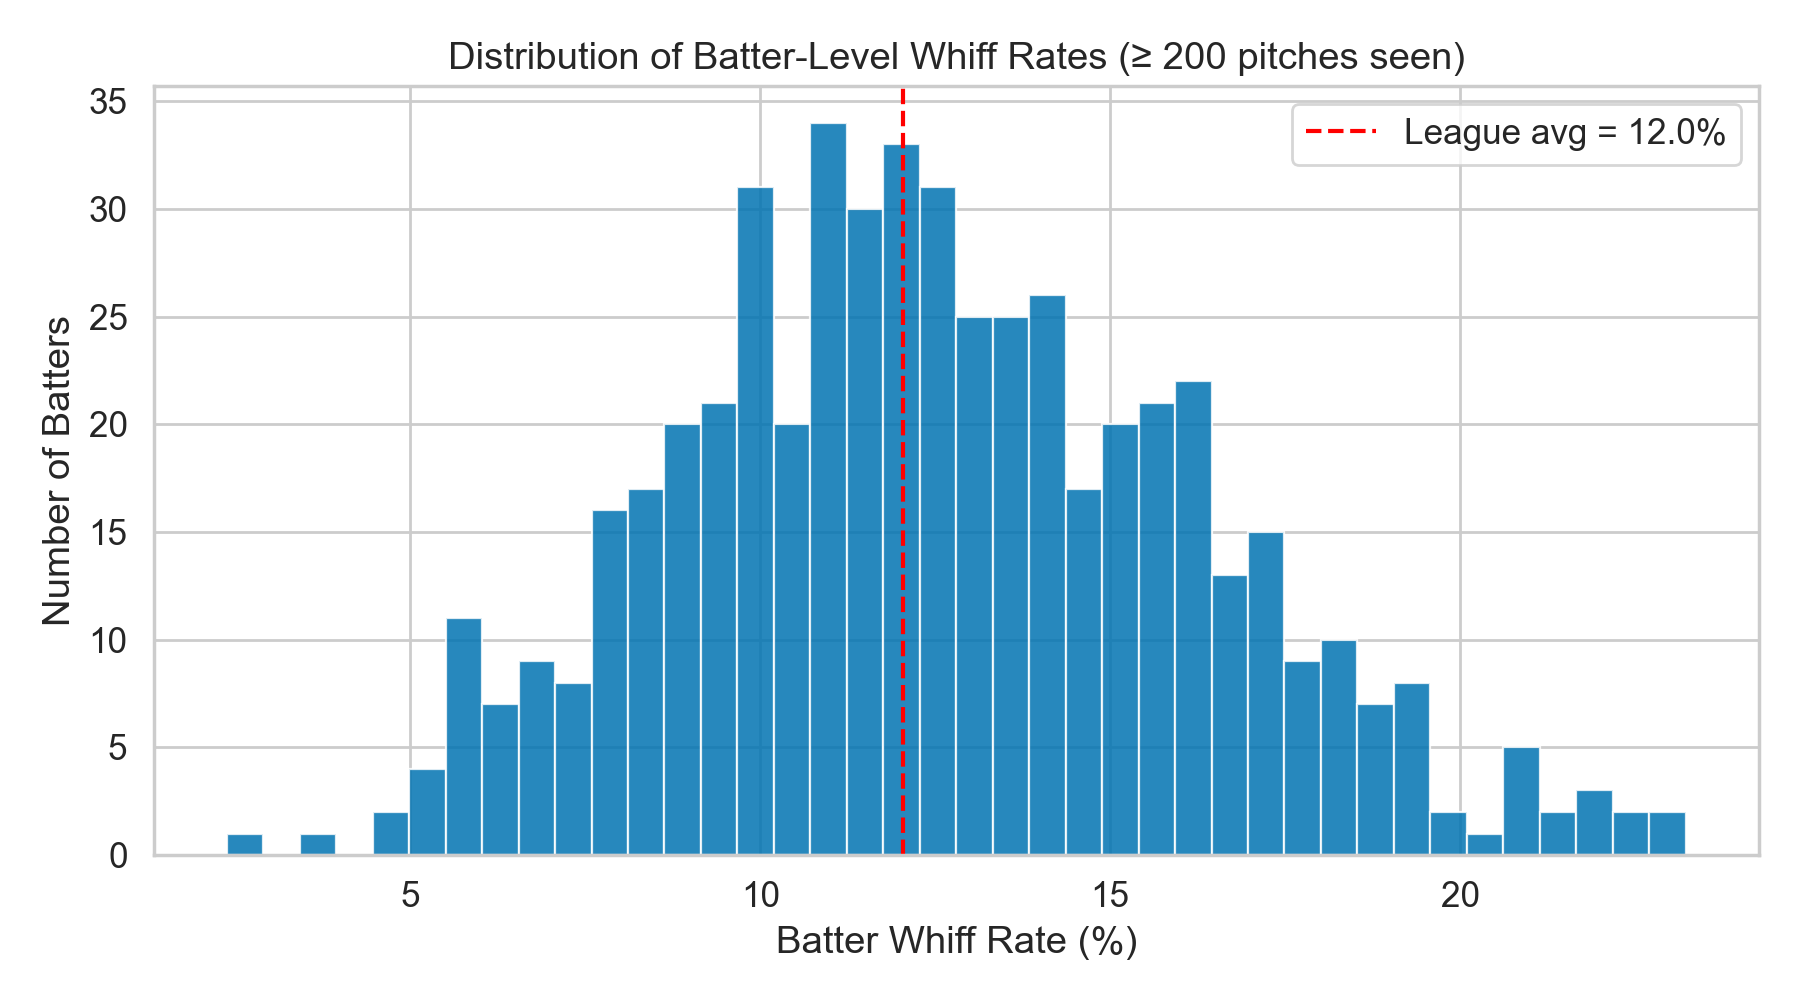
\includegraphics[width=0.8\textwidth]{figures/fig_batter_whiff_dist.png}
    \caption{Distribution of batter-level whiff rates (batters with $\geq 200$ pitches seen). The dashed red line marks the overall league whiff rate. Substantial heterogeneity motivates the use of batter random effects.}
    \label{fig:batter_dist}
\end{figure}

\subsection{Predictor Correlations}

Figure~\ref{fig:corr} presents the pairwise correlations among the continuous predictors and the binary whiff outcome.
Release speed and induced vertical break are positively correlated, largely because high-velocity fastballs also tend to have higher vertical break.
Horizontal break shows weaker correlations with the other predictors.
None of the individual correlations with the whiff outcome are strong in magnitude, which is consistent with our earlier observation that no single physical characteristic is a dominant predictor of swing-and-miss outcomes.
The relatively modest inter-predictor correlations suggest that multicollinearity is unlikely to be a concern in the logistic regression models.

\begin{figure}[H]
    \centering
    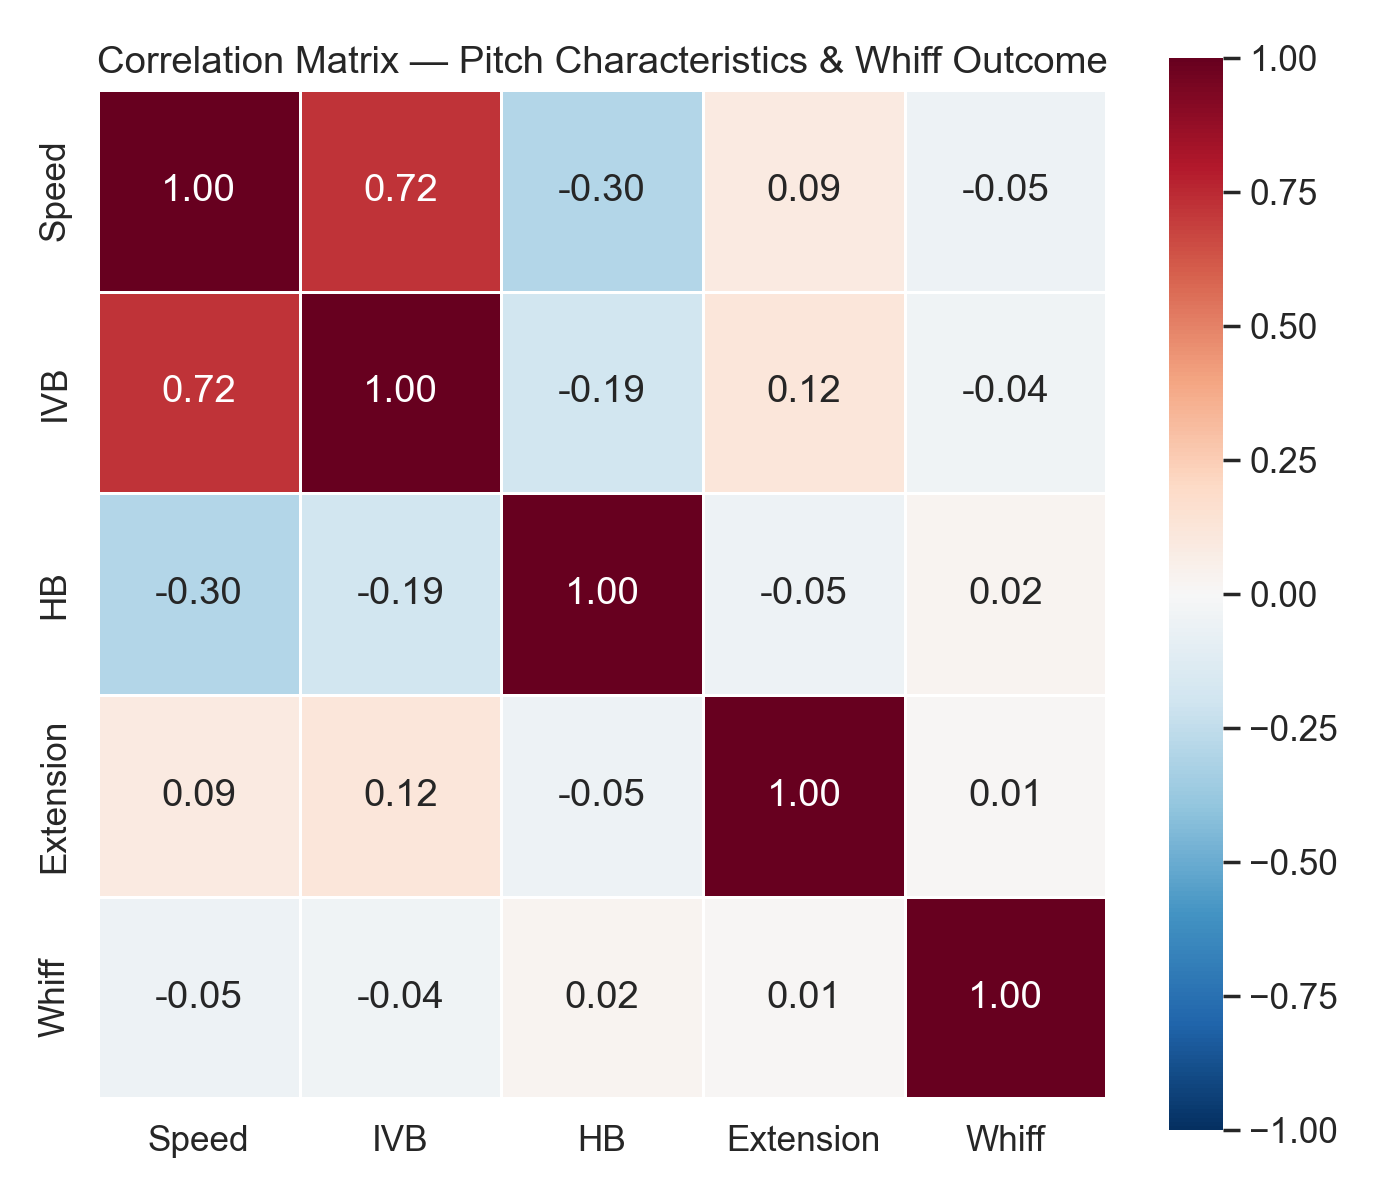
\includegraphics[width=0.6\textwidth]{figures/fig_correlation_matrix.png}
    \caption{Correlation matrix of continuous pitch characteristics and the binary whiff outcome. Correlations with whiff are small in magnitude, supporting the need for richer models.}
    \label{fig:corr}
\end{figure}

%%==============================================================
\section{Discussion and Next Steps}
%%==============================================================

The exploratory analysis reveals several findings that inform our modeling strategy.
First, whiff rates vary substantially across pitch types, with breaking balls and off-speed pitches generating the most swing-and-miss outcomes.
Second, pitch sequencing appears to matter: fastball-to-breaking-ball transitions show elevated whiff rates relative to baseline, consistent with the pitch tunneling hypothesis.
Third, batter-level whiff rates span a wide range, confirming that batter identity is an important source of variation that should be accounted for in modeling.
Fourth, no single physical pitch characteristic dominates the prediction of whiff outcomes, underscoring the need for multivariate models that incorporate both pitch-level and context-level information.

In the next phase of this project, we will proceed with the three-model framework outlined in the introduction:
\begin{enumerate}[nosep]
    \item A \textbf{baseline logistic regression} using physical pitch characteristics only (Equation~\ref{eq:baseline}),
    \item A \textbf{sequencing model} that adds lagged pitch variables and pitch-type interactions, and
    \item A \textbf{GLMM} that incorporates batter random intercepts.
\end{enumerate}
We will compare these models using likelihood ratio tests, BIC, and out-of-sample predictive accuracy to determine whether sequencing and batter heterogeneity provide meaningful improvements over the baseline.


%% BIBLIOGRAPHY
%%==============================================================
\newpage
\bibliographystyle{chicago}
\bibliography{Report1Ref}

\end{document}
